\documentclass{article}
\usepackage[pdftex]{graphicx}
\usepackage[export]{adjustbox}
\usepackage{amsmath}
\usepackage{amssymb}
\usepackage[dutch]{babel}
\usepackage{fullpage}
\usepackage{epsfig}
\usepackage[T1]{fontenc}
\usepackage{epstopdf}
\usepackage{relsize}
\newcommand{\zv}{\blacksquare}
\newcommand{\wv}{\square}
\newcommand{\R}{\mathbb{R}}
\newcommand{\N}{\mathbb{N}}
\usepackage{float}
\usepackage[caption = false]{subfig}
\usepackage{graphicx}
\usepackage{tikz}
\usetikzlibrary{matrix}
\begin{document}

\title{Elliptische Kromme Diffie-Hellman}

\author{R.L. Neuteboom (4006712) S.E.M.P. Franssen(4035844)\\
\small Universiteit Utrecht \normalsize}

\date{\today}
\maketitle
\section{Inleiding}
Tegenwoordig is het steeds belangrijker om communicatie die via het internet wordt verspreid te versleutelen. Zelfs als informatie nietszeggend lijkt te zijn, kunnen mensen die de gegevens onderscheppen veel daaruit opmaken. Een voorbeeld hiervan heb ik gezien bij een gastcollege van het vak Databases. Hier liet de gastspreker zien dat je op basis van geringe informatie over \'e\'en persoon, vaak relatief eenvoudig uit een grote database een kleine groep kan aanwijzen waar die persoon zich in bevindt. Zolang er geen technische ingreep nodig is om bij de gegevens te komen, kun je in Nederland nog veel verkeer legaal afluisteren.(Pas deze regel aan naar hoe het wel klopt)\\
In dit verslag wordt beschreven hoe je het Diffie-Hellman protocol kunt gebruiken om versleutelde communicatie op te zetten. Voor dit protocol is een systeem nodig om in te werken. Het systeem dat we gebruiken, zal bestaan uit een eindige cyclische multiplicatieve groep. We cre\"eren deze met behulp van een elliptische kromme. Verder willen we het bericht ondertekenen, dit zodat de ontvanger weet dat het van ons komt. Het kan namelijk zo zijn dat iemand anders contact probeert te zoeken met de ontvanger en valse berichten stuurt. Ten slotte gaan we in op hoe we deze technieken/algoritmen hebben ge\"implementeerd in Python.
\section{Diffie-Hellman protocol}
Het Diffie-Hellman protocol is een manier om een sleutel af te spreken die vervolgens gebruikt kan worden voor versleutelde communicatie. De effectiviteit van het protocol is gebaseerd op het feit dat een bepaalde bewerking niet makkelijk om te keren is, bijvoorbeeld multiplicatie in een bepaalde groep.\\
De bedoeling is dat een bericht van A naar B gestuurd kan worden, zonder dat anderen, E, die het bericht onderscheppen het kunnen begrijpen. Dit is het principe van Cyptografie. Binnen de Cryptografie is het standaard  dat A met Alice, B met Bob en de afluisteraar met Eve wordt aangeduid. Als ergens in de tekst het woord \emph{openbaar} wordt gebruikt, komt dat neer op dat ervan uit moet worden gegaan dat derden ook die informatie ontvangen en kunnen lezen.
Het Difie-Hellman protocol gaat als volgt te werk:
\begin{itemize}
\item Alice en Bob communiceren in het openbaar, dus afluisterbaar, het systeem dat ze gaan gebruiken om de sleutel van latere communicatie te bepalen. In ons verhaal is dit door middel van Elliptische Krommen. Hierbij leggen Alice en Bob een kromme, een basispunt op die kromme vast en een priemgetal af.
\item Alice en Bob bedenken afzonderlijk van elkaar een priv\'{e}sleutel.
\item Alice en Bob vermenigvuldigen hun priv\'{e}sleutel met het punt van de elliptische kromme en sturen het resultaat naar elkaar op.
\item Vervolgens vermenigvuldigen beiden hun priv\'{e}sleutel met het ontvangen punt. Alice en Bob hebben nu een gedeeld geheim (dat punt maal beide priv\'esleutels) die ze kunnen gebruiken voor versleutelde communicatie.
\end{itemize}
Naast elliptische krommen kan ook iets anders worden  gekozen. Zolang het iets is waarop je een bewerking kan doen die moeilijk om te keren is en dat het een associatieve commutatieve bewerking is.\\
Het protocol kan ook nog eens worden uitgebreid naar meer personen. Dit uitgebreide protocol werkt als volgt: elk van de personen kiest een priv\'esleutel. 
Het geheim wordt het basispunt maal \emph{alle} priv\'esleutels. Vervolgens wordt er heen en weer gecommuniceerd en krijgt ieder het basispunt maal alle priv\'esleutels, uitgezonderd de zijne te weten. Op deze manier is het nog steeds zo dat afluisteraars alleen maar weten wat het punt maal een aantal, maar niet alle, priv\'esleutels is.  
We gaan ervan uit dat Eve alle communicatie onderschept en precies weet wat we aan het doen zijn. Het enige van dit verhaal wat zij niet weet zijn de priv\'{e}sleutels en het gedeelde geheim.
Het is voor Eve genoeg om achter \'{e}\'{e}n van de priv\'{e}sleutels te komen, met deze kan ze namelijk achter het gedeelde geheim komen. De veiligheid van het systeem hangt dus af hoe moeilijk het is om gegeven het punt en het punt bewerkt met een van de priv\'{e}sleutels erachter te komen wat de priv\'{e}sleutel is.\\
Omdat we werken in een eindige groep waarbij er voor het omkeren van de bewerking geen algortime is, hangt de moeilijkheidsgraad van het oplossen van dat probleem af van de orde van de groep.

\section{Elliptische Krommen}
Het Diffie-Hellman protocol kan gebruik maken van Elliptische Krommen. Voor we bespreken hoe dat kan, stellen we vast wat Elliptische Krommen zijn. \\
Een elliptische kromme is een kromme die beschreven kan worden met punten $(x,y)\in\mathbb{R}^2$ die voldoen aan:
\begin{equation}
y^2 = x^3 + ax +b.
\end{equation}
Om een bruikbare Elliptische Kromme te hebben moeten we de voorwaarde stellen dat zijn grafiek non-singulier is. De definitie van singulier hangt af van het type grafiek wat bestudeerd wordt. Voor dit type grafiek betekent singulier dat de grafiek voldoet aan de volgende eisen:
\begin{itemize}
\item De grafiek heeft geen zelfintersecties.
\item De punten van de grafiek: $E$ moet beschreven kunnen worden met een bijectieve parametrisatie, oftwel $\exists p \in C(\mathbb{R},E)$ bijectief.
\item De parametrisatie moet de afgeleide overal gedefinieerd zijn en ongelijk aan nul. 
\end{itemize}
Op de grafiek van een elliptische kromme zijn we ge\"interesseerd in punten $(x,y)\in \mathbb{Z}^2$. Om te zorgen dat de kromme daar ook punten in heeft, eisen we dat $(a,b)\in\mathbb{Z}$. Reden hiervoor is dat we met de net besproken grafiek een eindige groep maken. We defini\"eren de groep $G$ dan op de volgende manier, een punt op de grafiek met gehele $x$ en $y$ is een element van onze groep. Het eenheidselement, aan te geven met $\infty$, is echter een punt dat niet op de grafiek ligt. Je zou het punt $\infty$ kunnen zien als het toegevoegde punt voor one-point-compactification.(Dat klopt toch?) De groepsoperatie '$+$' op punten $A$ en $B$ is op de volgende manier gedefinieerd: \\
we trekken een lijn door $A$ en $B$, laat $C$ het andere snijpunt met de grafiek zijn. We spiegelen $C$ in de $x$-as en het resultaat is $A+B$. Zie ook figuur \ref{optellen}.\\
\begin{figure}[H]
\center
\includegraphics[scale=0.3]{add-points-example.png}
\caption{Optelling van punten op Elliptische Krommen, bron jeremykunblabla.}\label{optellen}
\end{figure}
Er zijn hierbij een aantal zaken nog onbesproken. Een punt bij zichzelf optellen is niet goed gedefinieerd met de definitie van daarnet, we defini\"eren de lijn met de raaklijn en dan werkt het wel. Dat die raaklijn een snijpunt heeft met de curve zou aangetoond kunnen worden met de stelling van B\'ezout (BRON jeremykunblablabl).\\
De stelling van B\'ezout gaat over het aantal gemeenschappelijke punten van twee algebra\"ische krommen. De stelling komt uit de algebra\"ische meetkunde, hier zijn wij echter te onbekend mee om deze stelling en het bijbehorende bewijs in dit verslag te verwerken. \\
Als we een punt bij zijn x-as spiegeling optellen is er geen derde punt op de kromme, we defini\"eren dat in de x-as spiegelen neer komt op vermenigvuldigen met $-1$ en uit die optelling komt dan ook $\infty$. \\
Iets wat in het vorige hoofdstuk genoemd was maar nog niet aangetoond is dat de optelling associatief en commutatief moet zijn. Dat de optelling van punten op de elliptische kromme commutatief is, is snel te zien als je naar de definitie kijkt van de optelling. Om te laten zien dat de optelling associatief is moet ook de stelling van B\'ezout worden gebruikt helaas moeten we het bewijs hiervan ook achterwege laten.
\subsection{Eindige velden}
Zoals we eerder vermeld hadden willen we een \emph{eindige} groep hebben, dat is de groep hierboven besproken niet of hij bevat alleen $\infty$ wat ook niet nuttig is. De manier waarop we dat doen is de waarden van $x$ en $y$ beperken tot een eindig lichaam, waarbij alleen gehele getallen zitten. Een lichaam is een verzameling met daarbij een multiplicatie, additie, subtractie en divisie.\\
Een eindig lichaam $F$ heeft de volgende eisen:
\begin{itemize}
\item $F$ moet gesloten zijn in de multiplicatie en additie, d.w.z. als je twee elementen van $F$ optelt of vermenigvuldigt is dit weer een element van $F$.
\item er is associativiteit van optelling en vermenigvuldiging: $\forall a,b\in F$ geldt $a +(b + c)= (a + b) + c$ en $(a \cdot b) \cdot c = a \cdot (b \cdot c)$.
\item commutativiteit van optelling en vermenigvuldiging: $\forall a,b\in F$ geldt $a + b= b + a$ en $a \cdot b = b \cdot a$.
\item er zijn eenheidselementen van optelling en vermenigvuldiging: $e_+, e_*$.
\item er zijn additieve en multiplicatieve inversen: $\forall a \in F, \exists a^{-1}_+,a^{-1}_*\in F$ zodanig dat $a + a^{-1}_+=e_+$ en $a \cdot a^{-1}_* = e_*$.
\item distributiviteit van vermenigvuldiging over optelling: $\forall a,b,c \in F$ geldt $a \cdot (b + c) = (a \cdot b) + (a \cdot c)$ en $(a+b)\cdot c = (a \cdot c) + (b \cdot c)$.
\end{itemize}
Het lcihaam dat wat we gaan gebruiken is $\mathbb{F}_p$, ook wel $\mathbb{Z}/p$. Ofwel de gehele getallen modulo $p$. Gegeven dat $p$ priem is voldoet $\mathbb{F}_p$ aan de eisen. Wat verder nog op te merken valt is dat we hierop ook geheeltallige machtsverheffing kunnen uitvoeren.
\subsection{Samenvoegen Elliptische Kromme met eindig veld}
De manier waarop we deze begrippen samenvoegen is door de normale groep van de Elliptische Krommen te gebruiken met \'e\'en verschil: $x$ en $y$ worden met hun respresentant (kleinste positieve waarde) uit de equivalentieklasse uitgedrukt. Het lijkt misschien gek dat dit kan, maar als we formules hebben die de rol overnemen van de lijnen trekken maakt het daarbij niet uit of we in een eindig lichaam of in de gehele getallen werken.\\
Dan moeten we uiteraard wel formules hebben.
Laten we eerst proberen een formule te construeren die ervoor zorgt dat we twee verschillende punten bij elkaar op kunnen tellen.
Stel we tellen $(x_A,y_A)$ bij $(x_B,y_B)$ op, met als $x_A=x_B$ dan $y_B\neq -y_A,y_A$. We moeten een lijn trekken, dat is de volgende lijn:
\begin{equation}
L(x) = \frac{y_A - y_B}{x_A - x_B} (x - x_B) + y_b 
\end{equation}
Om aan het andere snijpunt te komen hoeven we alleen maar de andere wortel van de volgende vergelijking te vinden:
\begin{equation}
(L(x))^2 = x^3 + ax + b 
\end{equation}
Omdat we de twee andere wortels al hebben kunnen we dit gemakkelijk oplossen met Vieta's formule.
Volgens die formule geldt het volgende:\\
Als je een polynoom van de vorm $$\sum_{k=0}^n a_kx^k$$ hebt, geldt als $\{x_1,x_2,...,x_n\}$ de wortels van die polynoom zijn (inclusief dubbele): $$\sum_{k=1}^n x_n =-\frac{a_{n-1}}{a_n}.$$
Ofwel bij deze formule hoeven we alleen nog maar de co\"efficient van $x^2$ te vinden. Als we dit uitwerken hebben we $$a_2 = (\frac{y_A - y_B}{x_A - x_B})^2$$ dus $$x_C = (\frac{y_A - y_B}{x_A - x_B})^2 - x_A - x_B.$$ De bijbehorende $y_C$ krijgen we door hem in te vullen: $$y_C= \frac{y_A - y_B}{x_A - x_B} (((\frac{y_A - y_B}{x_A - x_B})^2 - x_A - x_B) - x_B) + y_b $$
(TODO zelfde maar met afgeleide)

\section{Ondertekenen}
Voor het ondertekenen van de berichten gebruiken we een HMAC (Hash-based Message Authentication Code). Voor HMAC is een cryptografisch veilige hash-functie nodig, hiervoor gebruiken we SHA256. Anders dan bij gebruikelijke hashfuncties zijn deze gemaakt op zo'n manier dat het erg moeilijk is om twee inputs te vinden die dezelfde output geven, daarnaast moet de input niet te achterhalen zijn. De input die wij gebruiken is de versleutelde tekst. 
\section{Implementatie: chat applicatie}
Om een chat applicatie te maken hebben we het volgende gedaan:
We hebben een onversleutelde chatapplicatie (server en client) gekopieerd van het internet om later aan te passen, een paar klassen geschreven om met de elliptische krommen om te gaan en als laatse  een klasse om te versleutelen en ontsleutelen van de tekst met AES geschreven.\\
ruw bestandenoverzicht:\\
\begin{itemize}
\item AES.py de inhoud van dit bestand wordt gebruikt voor AES encryptie en decryptie.
\item EC.py wordt gebruikt om te defini\"eren wat een punt, curve en finite field is.
\item crypto.py is verantwoordelijk voor het toepassen van AES op de tekst en het afspreken van de keys met Diffie-Hellman.
\item tcp.py is het serverprogramma, deze gebruikt bovenstaande bestanden om een connectie op te zetten en communiceert alles van de aangesloten clients door, dit doet hij door met elk van de clients Diffie-Hellman protocol af te gaan.
\item telnet.py is de client, deze moet communiceren met de server, weergeven wat er binnenkomt en ook weergeven wat je hebt getypt.
\end{itemize}
\subsection{diepere werking}
hieronder een overzicht van de klassen, bestanden en de relaties ertussen, een gerichte pijl betekent dat waar de pijl naar wijst gebruikt wordt door waar hij vandaan komt. Vervolgens gaan we in op hoe de communicatie verloopt tussen server en clients.

\begin{center}
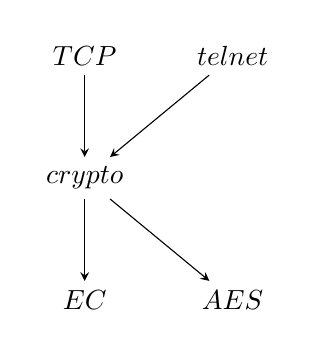
\begin{tikzpicture}
  \matrix (m) [matrix of math nodes,row sep=3em,column sep=2em,minimum width=2em]
  {
   TCP & telnet\\
   crypto \\
   EC & AES\\
   };
  \path[-stealth]

    (m-1-1) edge node [left] { } (m-2-1)
    (m-1-2) edge node [left] { } (m-2-1)
    
    (m-2-1) edge node [right] {} (m-3-1)

    (m-2-1) edge node [left] {} (m-3-2);   
\end{tikzpicture} 
\end{center}
Communicatie verloopt als volgt. Stel we verbinden als Client C met een server S. Als eerste stap zal de server alle andere gebruikers op de hoogte stellen dat er een nieuw iemand meeluistert, ook reageert de server met de eerste stap van het DH protocol op C. De Client stuurt zelf ook de eerste stap van het DH protocol op. Vervolgens berekenen de Server S als de Client C hun gedeeld geheim. Van dit geheim worden deelsleutels gemaakt die de up- en downstream van en naar de server beveiligen. Als C een bericht wil sturen aan de anderen die verbonden zijn met de server versleutelt C zijn bericht met de upstream keys naar de server. Vervolgens verstuurt C dit bericht naar de server. De server ontvangt dit bericht en ontsleutelt deze met de upstream key van C naar de server. Nu heeft de server het bericht dat C aan alle andere clients wilde sturen. Vervolgens genereert de server voor elke client $\tilde{C}$ een eigen versleuteling van het bericht met de downstream sleutels van $\tilde{C}$ naar de server. Vervolgens verstuurt de server dit bericht naar $\tilde{C}$. $\tilde{C}$ ontvangt dan dit bericht en kan met zijn downstream keys dit bericht ontsleutelen. 
\subsubsection{EC.py}
Dit bestand bevat alles wat nodig is om met de elliptische krommen te kunnen werken. De klasse FiniteFieldElem is ervoor om te zorgen dat er in het eindige lichaam gewerkt kan worden i.c.m. de elliptische kromme, heeft de variabele $p$ om $\mathbb{F}_p$ te kunnen vormen voor $p$ priem.\\ De klasse Curve heeft twee variabelen $a$ en $b$ zoals eerder om de kromme te defini\"{e}ren en $p$ om aan te geven op welk finitefield we werken.\\
De klasse Punt stelt een punt op een kromme voor, de variabelen x en y zijn FiniteFieldElem's, de klasse Eenheid is een subklasse van Punt en stelt het eenheidselement voor.
\subsubsection{AES.py}
Dit bestand zorgt ervoor dat tekst versleuteld kan worden d.m.v. AES. Als begin hebben we een implementatie van AES van het internet af geplukt die een blok van 16 bytes versleutelde met behulp van een 16 byte sleutel. Vervolgens hebben we deze code aangepast zodat hij een willekeurig lange stroom data kan versleuten, met behulp van codebookchaining. Deze module moet geinitialiseerd worden met een masterkey en een iv. De masterkey genereerd de rondesleutels, en deze moet elke sessie willekeurig gekozen worden of tot stand komen door een betrouwbaar key agreement protocol, en geheim blijven. De IV hoeft alleen willekeurig te zijn. Bij een gefixeerde IV, of niet willekeurig gekozen IV daald het aantal bericht die veilig versleuteld kunnen worden zonder collisies.
\subsubsection{Crypto.py}
Dit bestand bevat de klasse LSEC, wat defini\"eert op welke kromme en eindig lichaam we werken  en de klasse crypto.
De klasse crypto gebruikt zowel AES.py als EC.py, de laatste hiervan om een sleutel af te spreken. AES om de versleuteling van de berichten te doen. Na de versleuteling worden de berichten ondertekend met een HMAC gebaseerd op SHA256. Er is gekozen voor encrypt then sign omdat deze methode veel minder gevoelig is voor side channel aanvallen, en dezelfde theoretische veiligheid bied. \\Verder wordt in Crypto.py verzorgd dat als er een gemeenschappelijke sleutel is afgesproken er via herhaald hashen via pbkdf2 hmac veilige sleutels en IVs worden verzorgd voor de upstream en downstream van gegevens, de IV voor die streams en de sleutels om die streams te ondertekenen met behulp van HMAC.
\subsubsection{tcp.py}
tcp.py is de Python file met daarin de server code. Deze houdt alle users bij met hun keys, en als er een bericht binnenkomt dan stuurt de server dit bericht door naar alle andere users van de server. De server gebruikt crypto.py om de berichten te versleutelen en met de clients keys af te spreken.
\subsubsection{telnet.py}
De Python file telnet.py is de file  voor de client en zorgt hij verbinding kan leggen met de server en kunnen communiceren. De client heeft in tegen stelling tot de server geen verbinding met alle gebruikers van de server maar alleen met de server zelf. 


\section{Aanvallen}
We bespreken in deze sectie enkele aanvalsmogelijkheden die een aanvaller hebben om het verkeer te onderscheppen. Ten eerste kan iedereen verbinding maken met de server waarop er gecommuniceerd wordt en het gesprek afluisteren. Echter, als iemand verbinding maakt wordt dit bericht naar alle andere gebruikers gepushed en zijn alle gebruikers op de hoogte dat er iemand meeluisterd. Er zijn ook andere methoden waarop de gebruikers niet op de hoogte hoeven zijn dat er iemand mee luistert. Verder kan het protocol gemakkelijk worden aangepast dat mensen zich moeten identificeren via een wachtwoord voordat ze mee mogen luisteren. Dit vergt een paar kleine aanpassingen voor de communicatie zelf. Echter wordt het problematisch om jezelf bij de server te registreren als ongeregistreerde berichten negeert worden. Hier zal een middenweg in gezocht moeten worden.
\subsection{Man in the middle}
Een iemand zou zich kunnen voordoen als een betrouwbare Server door al het verkeer af te luisteren. Vervolgens kan deze persoon dit verkeer door sluizen naar de echte server en tegen de server doen alsof hij de Client is. Omdat ip-pakketten vervalst kunnen worden kan dit worden gedaan zonder dat de gebruikers er iets van merken. 
\subsection{Server omkopen}
Omdat al het verkeer via de server wordt geleid en de server over alle keys beschikt, kan een kwaadwillende server al het verkeer prijsgeven. 
\subsection{Side channel aanvallen}
Onze server is niet beveiligd tegen alle sidechannel aanvallen. Onze DH suite is licht gevoelig voor timing aanvallen en die zou gebruikt kunnen worden om de interne staat van de klasse random te verraden. De klasse random is niet cryptografisch veilig en iemand kan daarmee gegevens over de geheime sleutel van de Client bemachtigen. Deze geven dan de mogelijkheid om de gedeelde sleutel te bemachtigen want met de geheime sleutel en de publieke transactie kan alles worden afgeluisterd.
\\Na de Key-Exchange zijn er geen side channel aanvalmogelijkheden bekend die van een afstand uit te voeren zijn. We gebruiken encrypt-then-sign omdat deze robuuster is tegen side channel aanvallen.
\subsection{Theoretische aanvallen}
Er bestaan ook aanvallen tegen AES en DH. Deze aanvallen zijn puur theoretisch op dit moment en zijn niet praktisch haalbaar. Als het discrete logarithme probleem wordt opgelost zou dit een flinke klap zijn voor de veiligheid van versleutelings algoritmen gebaseerd op Diffie-Hellman sleutel uitwisseling. Echter zijn elliptische krommen resistanter dan andere varianten van het Diffie-Hellman protocol. Verder zou het kunnen dat AES gebroken wordt en er een ciphertext aanval komt. Dit is echter onwaarschijnlijk aangezien AES een goed onderzocht protocol is, gebaseerd op wiskundig goed onderbouwde methoden. Ten derde zou men een aanval tegen bijvoorbeeld SHA256 kunnen vinden zodat de message authenticatie vervalst kan worden en mensen daarna side channel aanvallen tegen gewoon cbc AES gaan doen via adaptive chosen ciphertext. Dit is echter moeilijker omdat de code die we geschreven hebben geen resultaat terug geeft over hoe lang het duurde om alles te ontsleutelen en of de ontsleuteling gelukt is. Dus via deze methode kun je ook geen delen van de data terugvinden.
\section{Conclusie}
We hebben in dit project een applicatie geschreven waarbij men redelijk veilig kan communiceren over het internet. Als een user eenmaal veilig de verbinding tot stand heeft gebracht kan men moeilijk het verkeer af luisteren. De optie om de servereigenaar af te kopen en de geheimen prijs te geven blijft echter altijd bestaan. Een manier om dit te voorkomen is de server en een van de clients op dezelfde computer te draaien en via andere communicatie af te spreken wie de server beheert.
\section{gebruikte bronnen}
http://www.binarytides.com/code-chat-application-server-client-sockets-python/\\
https://github.com/bozhu/AES-Python\\
Weisstein, Eric W. "Field Axioms." From MathWorld--A Wolfram Web Resource.\\ http://mathworld.wolfram.com/FieldAxioms.html \\
en andere eventuele bronnen vermeld in de Python3 bestanden.
\end{document}
